\subsection{UCE1 - Visualizzazione errore informazioni utente}\label{usecase:e_1}
\begin{figure}[H]
    \centering
    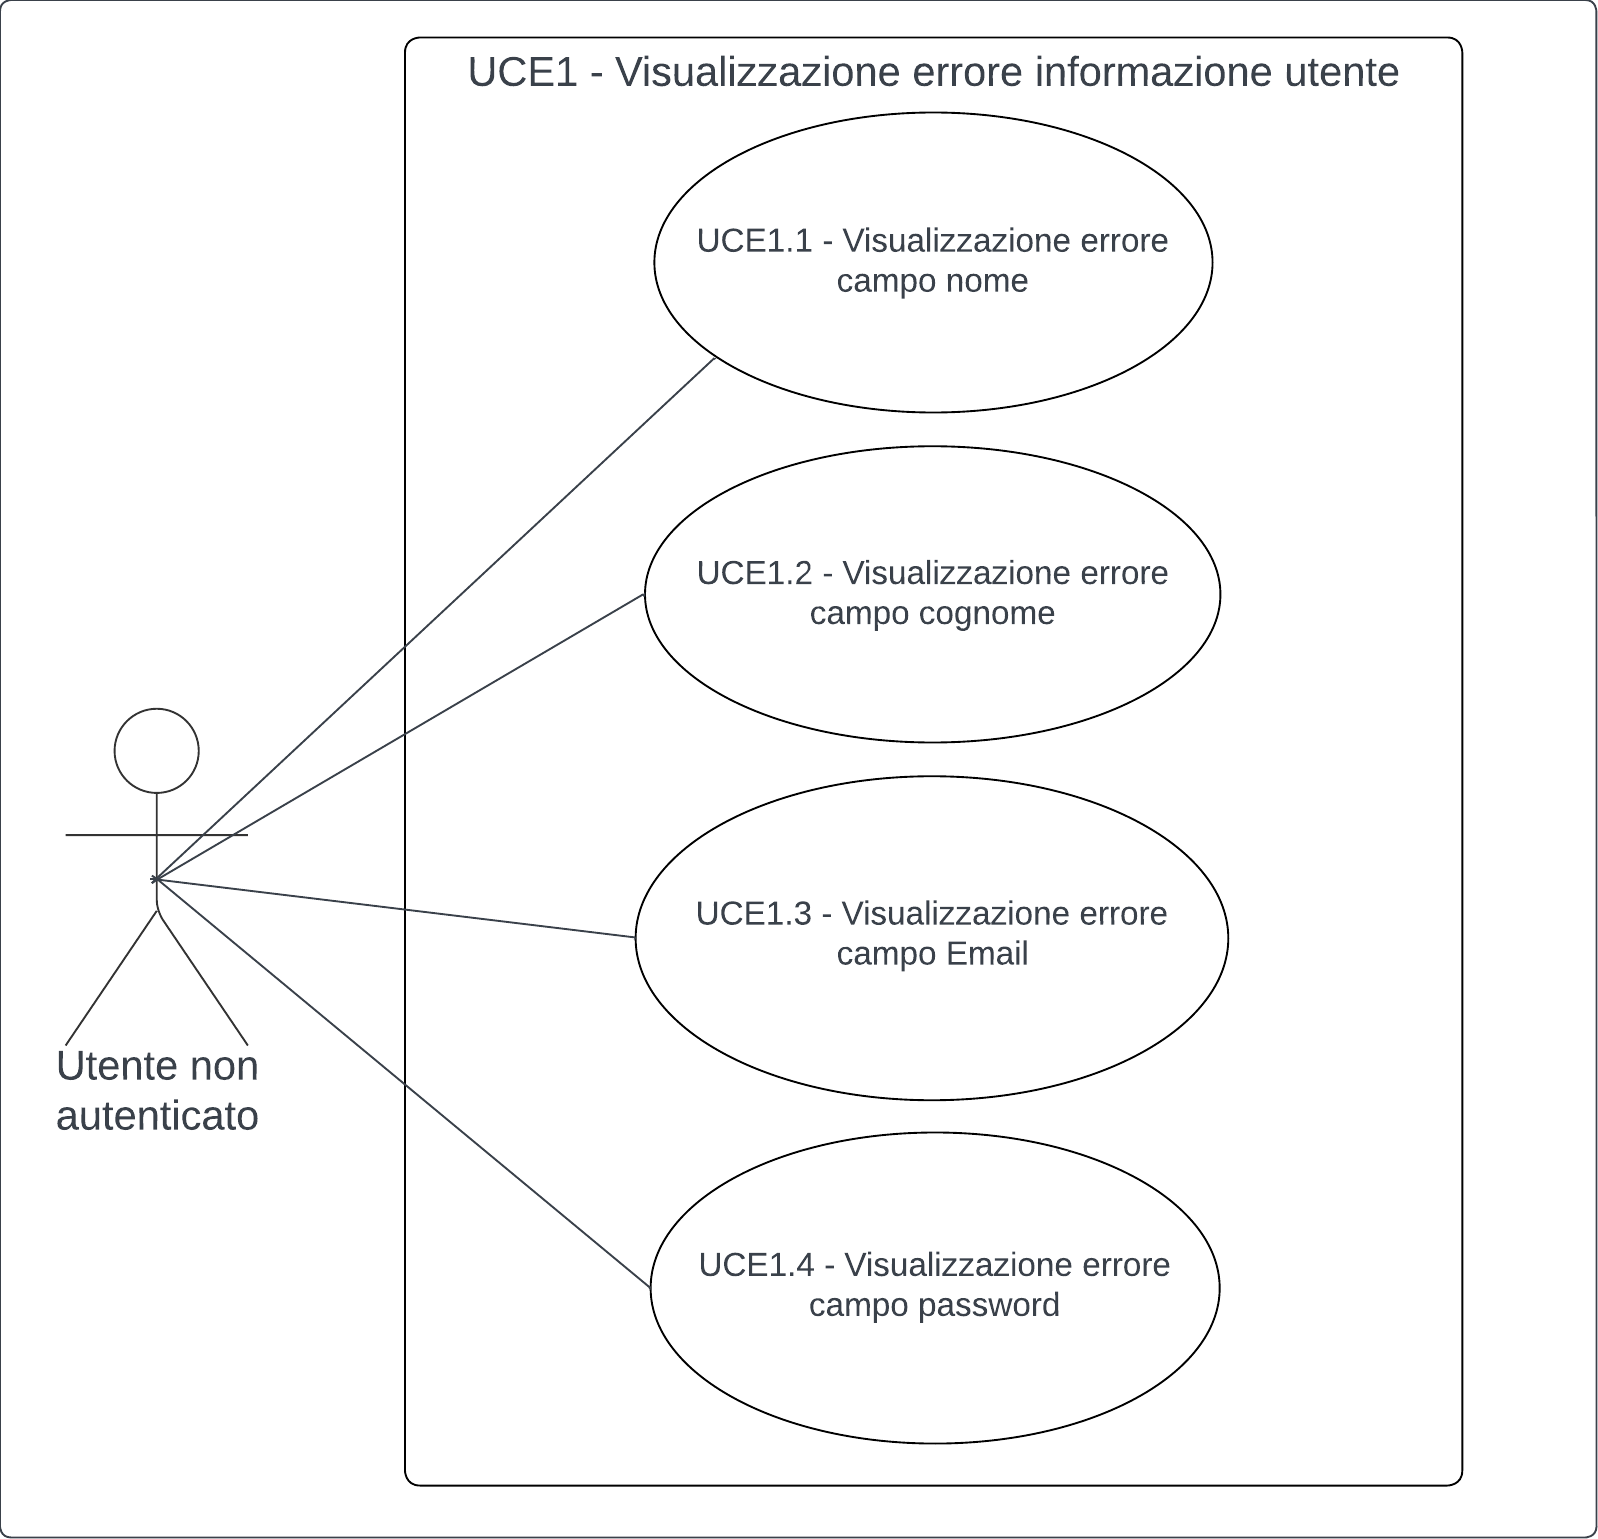
\includegraphics[width=0.75\linewidth]{ucd/UCED1.png}
\end{figure}
\textbf{Attori}:
\begin{itemize}
    \item Attore non autenticato
\end{itemize}
\textbf{Precondizioni}:
\begin{itemize}
    \item L'utente ha inserito in modo errato una o più dei seguenti campi:
    \begin{itemize}
        \item username
        \item email
        \item password
    \end{itemize}
\end{itemize}
\textbf{Postcondizioni}:
\begin{itemize}
    \item L'utente visualizza un messaggio di errore che specifica cosa ha sbagliato
\end{itemize}
\textbf{Scenario principale}:
\begin{enumerate}
    \item L'utente visualizza un errore che specifica quale campo non è conforme a quanto richiesto
    \item L'utente può modificare il campo sbagliato
\end{enumerate}
\textbf{Scenario alternativi}:
\begin{enumerate}
    \item L'utente sceglie di annullare la procedura di inserimento dati
\end{enumerate}
\subsubsection{UCE1.1 - Visualizzazione errore campo nome}
\begin{figure}[H]
    \centering
    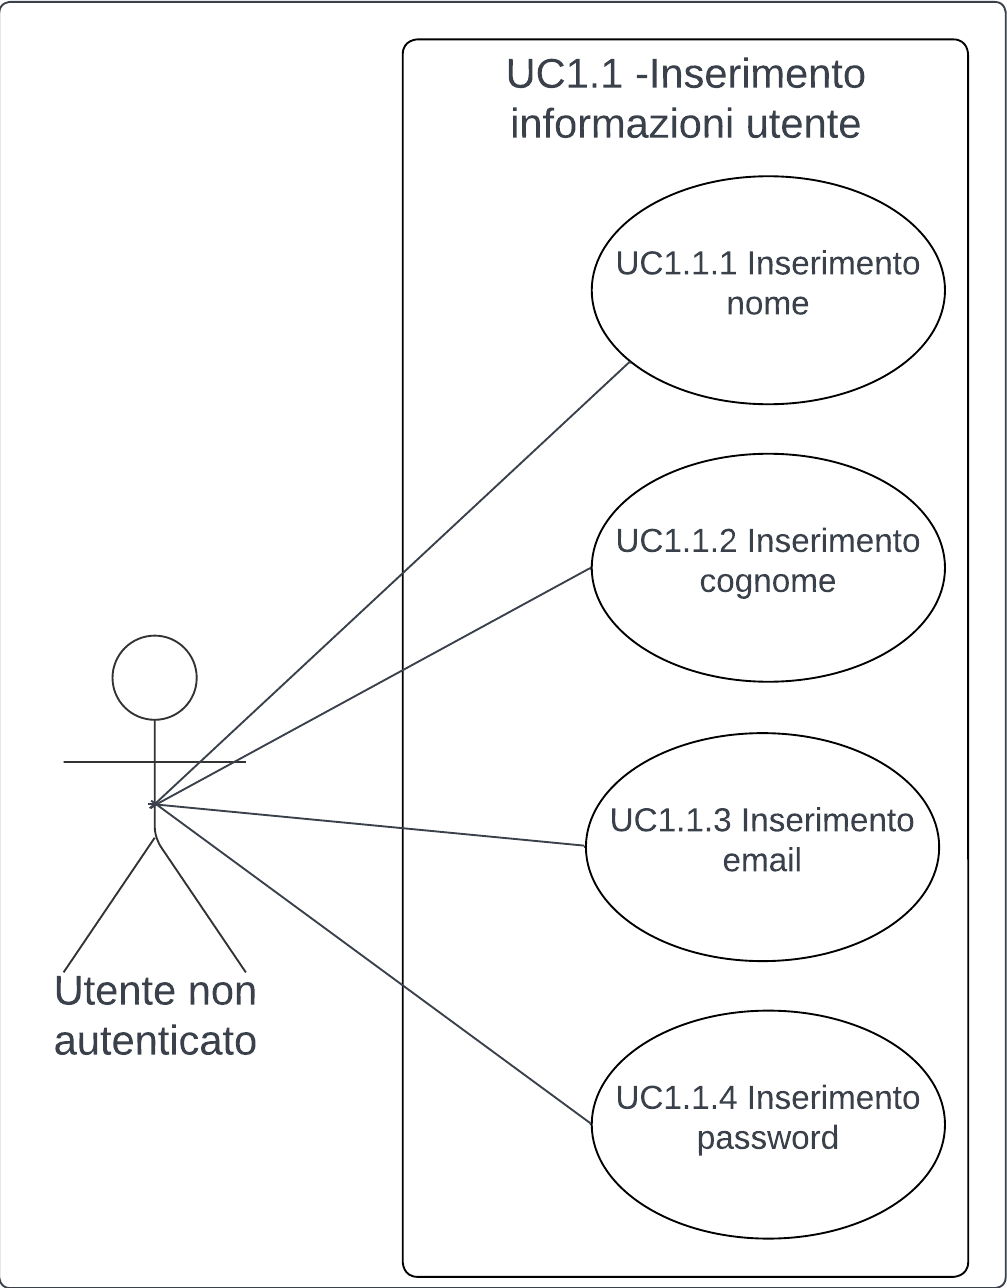
\includegraphics[width=0.75\linewidth]{ucd/UCD1.1.png}
\end{figure}
\textbf{Attori}:
\begin{itemize}
    \item $\textit{Attore}_G$ non autenticato.
\end{itemize}
\textbf{Precondizioni}:
\begin{itemize}
    \item L'utente ha inserito un nome non valido.
\end{itemize}
\textbf{Postcondizioni}:
\begin{itemize}
    \item L'utente visualizza un messaggio di errore e $\textit{sistema}_G$ corregge l'errore.
\end{itemize}
\textbf{Scenario principale}:
\begin{enumerate}
    \item L'utente visualizza un errore;
    \item L'utente modifica il campo sbagliato.
\end{enumerate}
\textbf{Scenario alternativi}:
\begin{enumerate}
    \item L'utente sceglie di annullare la procedura di inserimento dati.
\end{enumerate}
\subsubsection{UCE1.2 - Visualizzazione errore campo cognome}
\textbf{Attori}:
\begin{itemize}
    \item $\textit{Attore}_G$ non autenticato
\end{itemize}
\textbf{Precondizioni}:
\begin{itemize}
    \item L'utente ha inserito un cognome non valido
\end{itemize}
\textbf{Postcondizioni}:
\begin{itemize}
    \item L'utente visualizza un messaggio di errore e $\textit{Sistema}_G$ corregge l'errore
\end{itemize}
\textbf{Scenario principale}:
\begin{enumerate}
    \item L'utente visualizza un errore 
    \item L'utente modifica il campo sbagliato
\end{enumerate}
\textbf{Scenario alternativi}:
\begin{enumerate}
    \item L'utente sceglie di annullare la procedura di inserimento dati
\end{enumerate}
\subsubsection{UCE1.3 - Visualizzazione errore campo email}
\textbf{Attori}:
\begin{itemize}
    \item $\textit{Attore}_G$ non autenticato
\end{itemize}
\textbf{Precondizioni}:
\begin{itemize}
    \item L'utente ha inserito una email non valida
\end{itemize}
\textbf{Postcondizioni}:
\begin{itemize}
    \item L'utente visualizza un messaggio di errore e $\textit{sistema}_G$ corregge l'errore
\end{itemize}
\textbf{Scenario principale}:
\begin{enumerate}
    \item L'utente visualizza un errore 
    \item L'utente modifica il campo sbagliato
\end{enumerate}
\textbf{Scenario alternativi}:
\begin{enumerate}
    \item L'utente sceglie di annullare la procedura di inserimento dati
\end{enumerate}
\subsubsection{UCE1.4 - Visualizzazione errore campo password}
\textbf{Attori}:
\begin{itemize}
    \item \textit{Attore_G} non autenticato
\end{itemize}
\textbf{Precondizioni}:
\begin{itemize}
    \item L'utente ha inserito una password non valida
\end{itemize}
\textbf{Postcondizioni}:
\begin{itemize}
    \item L'utente visualizza un messaggio di errore e \textit{Sistema_G} corregge l'errore
\end{itemize}
\textbf{Scenario principale}:
\begin{enumerate}
    \item L'utente visualizza un errore 
    \item L'utente modifica il campo sbagliato
\end{enumerate}
\textbf{Scenario alternativi}:
\begin{enumerate}
    \item L'utente sceglie di annullare la procedura di inserimento dati
\end{enumerate}
\newpage